\documentclass[11pt]{article}
\usepackage[utf8]{inputenc}
\usepackage[czech]{babel}
\usepackage[unicode]{hyperref}
\usepackage{graphicx}
\usepackage[a4paper, total={17cm, 24cm}, left=2cm, top=3cm]{geometry}
\usepackage{fancyhdr}
\usepackage{minted}
\usepackage{hyperref}

\setlength{\headheight}{14pt}
\pagestyle{fancy}
\fancyhf{}
\rhead{Prokotol o řešení projektu ISS}
\lhead{Martin Zmitko (xzmitk01)}
\cfoot{\thepage}

\newcommand{\pic}[2]{
    \begin{figure}[h!]
    \centering
    \includegraphics[width=0.75\textwidth]{#1}
    \caption{#2}
    \end{figure}
}

\begin{document}
\section{Základy}
Projekt byl řešen v programovacím jazyce \texttt{Python} s použitím \texttt{Jupyter Notebook}, byly využity knihovny \texttt{Numpy}, \texttt{Scipy} a \texttt{Matplotlib}.
Signál byl načten pomocí funkce \texttt{scipy.wavfile.read} z knihovny jako \texttt{Numpy ndarray}. 
O signálu byly pomocí knihovních funkcí zjištěny následující údaje:
\begin{verbatim}
Samplerate: 16000
Number of samples: 54068
Length: 3.37925s
Minimal sample: -3101, Maximal sample: 3496
\end{verbatim}
\pic{img/1_signal.png}{Zobrazení zvukového signálu}

\section{Předzpracování a rámce}
Signál byl ustředněn a normalizován následovně:
\begin{minted}{python}
s = s - np.mean(s) #ustřednění
s = s / max(s.min(), s.max(), key=abs) #normalizace
\end{minted}

Následně byl signál rozdělen do rámců o délce 1024 vzorků a uložen do dvojrozměrného pole, přičemž jednotlivé rámce byly uloženy do sloupců.
Rozdělení do rámců proběhlo pomocí cyklu, ve kterém bylo do každého sloupce uloženo 1024 vzorků z aktuální polohy, která byla posunuta vždy o 512 vzorků, dokuď nebylo rozděleno celé pole.

Pro zobrazení byl vybrán 14. rámec, ve kterém je vyslovována samohláska \uv{e}.
\pic{img/2_frame.png}{Zobrazení 14. rámce signálu}

\section{DFT}
Vlastní funkce pro diskrétní fourierovu transformaci byla vytvořena pomocí funkce \texttt{scipy.linalg.dft}, která vytvoří matici pro dft o zadané velikosti (v tomto případě 1024) a následného maticového násobení této matice s rámcem signálu. 
Je zobrazena má implementace dft zároveň s funkcí \texttt{numpy.fft.fft} na 14. rámci signálu, oba grafy jsou vizuálně shodné.
\pic{img/3_dft.png}{Porovnání mé implementace dft a knihovní fft}

\section{Spektrogram}
Spektrogram s velikostí okna 1024 a překrytím 512 byl vytvořen pomocí funkce
\begin{minted}{python}
plt.specgram(s, window=None, Fs=fs, NFFT=1024, noverlap=512)
\end{minted}
\pic{img/4_spectrograph.png}{Spektrogram signálu}

\section{Určení rušivých frekvencí}
Rušivé frekvence byly určeny pomocí funkce \texttt{scipy.signal.find\_peaks} použité na první rámec signálu po fourierově transformaci.
Funkce vrátila následující hodnoty:
\begin{verbatim}
peaks = [ 703.125, 1406.25, 2109.375, 2812.5 ]
\end{verbatim}

Ověření, jestli jsou frekvence harmonicky vztažené bylo provedeno vydělením všech frekvencí tou nejnižší, výsledek byla celá čísla, frekvence jsou tedy násobky nejnižší.

\section{Generování signálu}
Signál byl vygenerovám pomocí sečtení 4 cosinusovek generovaných následovně:
\begin{minted}{python}
samples = np.arange(s.size) / fs
for i in range(4):
    cos += np.cos(2 * np.pi * peaks[i] * samples)
\end{minted}

Signál byl následovně uložen do souboru pomocí funkce \texttt{scipy.io.wavfile.write}.
Poslechem a pomocí spektrogramu bylo ověřeno, že byly rušivé frekvence určeny správně.
\pic{img/6_spectrograph.png}{Spektrogram signálu s rušivými cosinusovkami}

\section{Čistící filtr}
Byly vytvořeny 4 bandstop filtry f0 až f3 (od nejnížší frekvence k nejvyšší) s šíří závěrného pásma 30 Hz a rozptylem přechodu do propustného pásma 50 Hz na každé straně. K návrhu filtrů byla použita funkce \texttt{scipy.signal.buttord}, která vrátila správný řád filtru (4) a kritické frekvence, které byly předány funkci \texttt{scipy.signal.butter}, která vrátila samotné koeficienty filtrů:
\begin{verbatim}
f0: a[  1.    -7.6   25.57 -49.69  61.02 -48.47  24.33  -7.05   0.91]
    b[  0.95  -7.32  24.94 -49.09  61.03 -49.09  24.94  -7.32   0.95]
f1: a[  1.    -6.72  20.86 -38.68  46.76 -37.71  19.83  -6.23   0.9 ]
    b[  0.95  -6.48  20.34 -38.2   46.77 -38.2   20.34  -6.48   0.95]
f2: a[  1.    -5.34  14.59 -25.13  29.73 -24.5   13.87  -4.95   0.9 ]
    b[  0.95  -5.14  14.23 -24.82  29.73 -24.82  14.23  -5.14   0.95]
f3: a[  1.    -3.55   8.63 -13.18  15.54 -12.85   8.2   -3.29   0.9 ] 
    b[  0.95  -3.42   8.41 -13.02  15.54 -13.02   8.41  -3.42   0.95]
\end{verbatim}

Impulzní odezvy byly vytvořeny aplikováním filtrů pomocí funkce \texttt{scipy.signal.lfilter} na signál s jedničkovým impulzem na začátku o délce 75 vzorků.
\begin{figure}[h!]
\centering
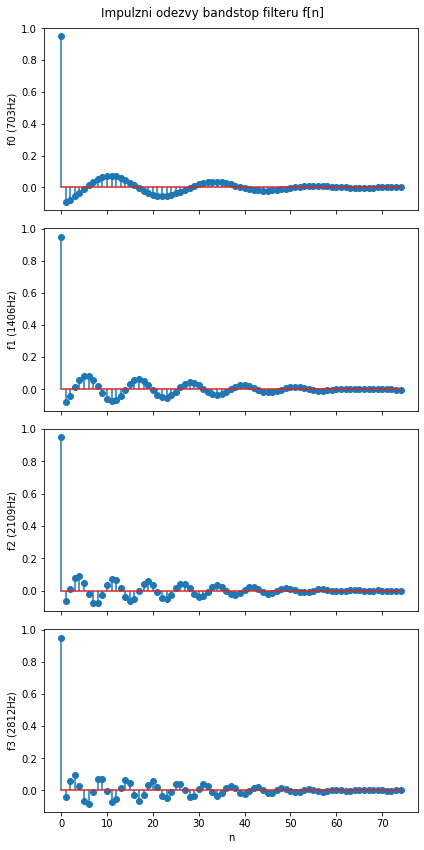
\includegraphics[width=0.6\textwidth]{img/7_impulse.png}
\caption{Impulzní odezvy navržených filtrů}
\end{figure}

\section{Nulové body a póly}
Nulové body a póly filtrů byly taktéž vypočítány pomocí funkce \texttt{scipy.signal.butter}, ale s parametrem \texttt{output='zpk'}.
\pic{img/8_coefs.png}{Nulové body a póly filtrů v komplexní rovině}

\section{Frekvenční charakteristika}
Frekvenční charakteristika byla vypočtena pomocí funkce \texttt{scipy.signal.freqz}.
\begin{figure}[h!]
\centering
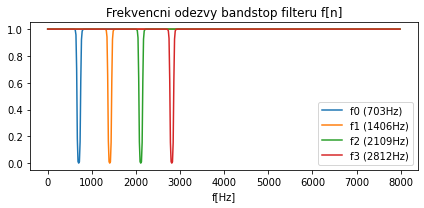
\includegraphics[width=0.9\textwidth]{img/9_freq_char.png}
\caption{Frekvenční charakteristika filtrů}
\end{figure}

\section{Filtrace}
Filtrace byla provedena použitím funkce \texttt{scipy.signal.lfilter} na signál pro každý filtr. 
Vypsáním největšího a nejmenšího vzorku bylo zjištěno, že je signál ve správném rozsahu $[-1, 1]$.
Výsledný signál byl uložen do souboru pomocí \texttt{scipy.io.wavfile}.

Poslechem bylo ověřeno, že rušivé frekvence byly odfiltrovány. 
Je ale slyšet, že se tyto frekvence z nahrávky ztratily a nahrávka je tedy mírně zkreslená.

\section{Použité zdroje}
\begin{itemize}
    \item Dokumentace numpy: \url{https://numpy.org/doc/1.21/}
    \item Dokumentace scipy: \url{https://docs.scipy.org/doc/scipy-1.7.0/reference/index.html}
    \item Dokumentace matplotlib: \url{https://matplotlib.org/stable/index.html}
\end{itemize}

\end{document}
